\documentclass[12pt,twoside]{article}
\usepackage{amsmath} 
\usepackage{fixltx2e}
\usepackage{enumerate}
\usepackage{url}
\usepackage{mdframed}
\usepackage{wrapfig}
\usepackage{graphicx}
\usepackage{float}

\input BoxedEPS


%%%%%%%%%%%%%%%%%%%%
%%
%% Depending on what operating system you are using, you need to
%% use one or other of the following two lines. Keep the one you
%% are NOT using ``commented out'', ie preceded by %.

\SetTexturesEPSFSpecial  %% use this for the Mac & Textures
%\SetRokickiEPSFSpecial  %% use for xdvi, dvips; i.e., for VMS, Unix, Athena

\HideDisplacementBoxes

\renewcommand{\baselinestretch}{1.2}
\setlength{\topmargin}{-0.2in}
\setlength{\textwidth}{6in}
\setlength{\textheight}{8.5in}
\setlength{\oddsidemargin}{0.25in}
\setlength{\evensidemargin}{0.25in}
\raggedbottom

\begin{document}

\title{Test automation framework design for Web Applications \\} 
\author{\\ Kamil Smuga\\
\small kamil.smuga@ieee.org\\ \\
\small COMP40070 Term Paper\\
\small School of Computer Science and Informatics\\
\small University College Dublin \date{\small\today} } 
\maketitle

\pagestyle{myheadings}
\markboth{Kamil Smuga}{High Availability in Modern Computer Architectures}
\thispagestyle{empty}

\begin{abstract}
\noindent

--- ABSTRACT --- \\ 
\end{abstract}

\section{Introduction}
 By definition, software is applied to automate processes that exist in a real world. To build software that solves complex problems we need software development process. Software development process contains software testing phase. When testing phase is applied differs between projects and methodologies. Whether testing will be performed manually or automatically depends on type of testing and number of other business and project specific factors. However, regression and acceptance tests are proven field to apply test automation. Test automation design is the subject of this paper.

\subsection{Domain Driven Design}
The vision of Domain Driven Design is being widely popularized by Eric Evans. Eric wrote popular book on the subject: \emph{Domain-Driven Design: Tackling Complexity in the Heart of Software}. In a nutshell, DDD refers to:
\begin{itemize}
\item [--] domain knowledge,
\item [--] model,
\item [--] ubiquitous language.
\end{itemize}
Each listed section applies differently to various context. The appliance in test automation is described below.

\subsubsection{Domain knowledge}
In order to create useful software, one needs to know what software is all about - must understand the domain. The entire purpose of the software is to enhance a specific domain. 
In software testing context, domain knowledge refers specifically to system under test (SUT) knowledge and understanding. A person who would be suitable is an experienced specialist with hands on experience on the product.  

\subsubsection{Model}
A model is essential part of the software design. All thinking process about the domain is synthesized into the model. The form of sharing model details can be: use case, diagram, drawing, picture or writing. 
Consider 2 people engaged in creating a model: test software designer --- responsible for designing a test automation framework --- and domain knowledge expert. They do not go into details but provide high level model of framework based on software behavior, as shown in the Figure \ref{model} below.  

\begin{figure}[H]
\centering
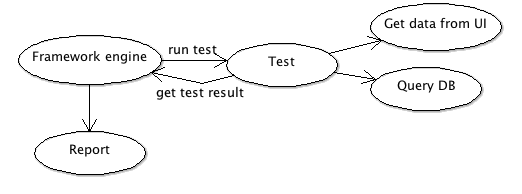
\includegraphics[width=120mm]{model.png}
\caption{Test automation software model}
\label{model}
\end{figure}

\subsubsection{Ubiquitous Language}
In order to develop model of the domain, domain experts have to work with test software designers. There is a quite realistic possibility of communication barrier -- software designer will think in terms of inheritance, polymorphism, OOP and domain expert will use product specific jargon. This indicates a necessity to create the same language. DDD principle suggest to use a language based on the model. This language is forced to use consistently in all forms of the communication - that is why is called the Ubiquitous Language. Furthermore, from a single test design perspective, it is crucial to express tests in the language of the end-user of application. This requirement leads to use keyword-driven framework, which details are explained below.   

\subsubsection{Keyword-driven framework}
Keyword-driven test design abstracts the implementation of tests behind high-level actions. In UI testing, keywords represents user basic actions such as pressing keys, clicking on application tabs, typing. The tests are build as sequences of keywords. Keywords are translated into low-level action implementations. This is hidden from test writer, which makes test easier to understand and create. An example of keyword-driven framework is Robot Framework - well-known open source project widely-used in the industry. The available keywords are defined in libraries: standard (i.e. BuiltIn, OperatingSystem, String) and external (i.e. Selenium, SSH, Swing, Database). Refer to Figure \ref{robot_tc} for test case example of jEdit file opening in Robot Framework.

\begin{figure}[H]
\centering
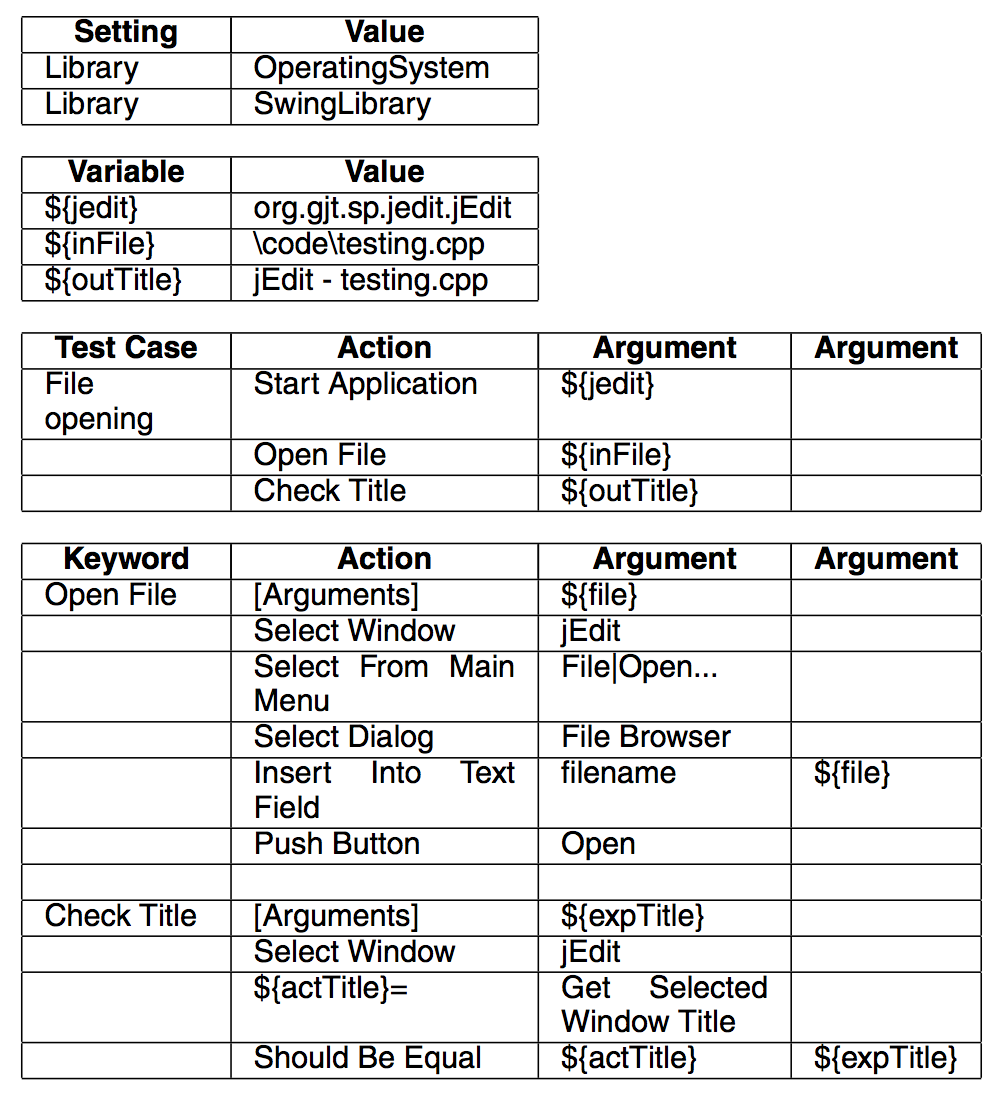
\includegraphics[width=120mm, height=140mm]{robot_tc.png}
\caption{An HTML format test data file including a test case
to test jEdit file opening in Robot Framework ~\cite{ref:2.1} }
\label{robot_tc}
\end{figure}

\subsubsection{Model-based testing}
One of the Model-based testing approaches is a generation of test cases with oracles from a behavior model. This can be seen as a specification-based test generation approach in which the model is the specification. This approach requires specific skill set from test designer --- from now will be called test modeler --- and good tool support. Good example of toolset is TEMA -- a set of model-based testing tools designed for domain-specific GUI application testing. The toolset provides a complete set of model-based testing tools from modeling to test generation. The authors of \emph{Model-Based Testing with a General Purpose Keyword-Driven Test Automation Framework} paper proved that integration of TEMA and Robot Framework is feasible and effective. For high level overview refer to Figure \ref{integration}.

\begin{figure}[H]
\centering
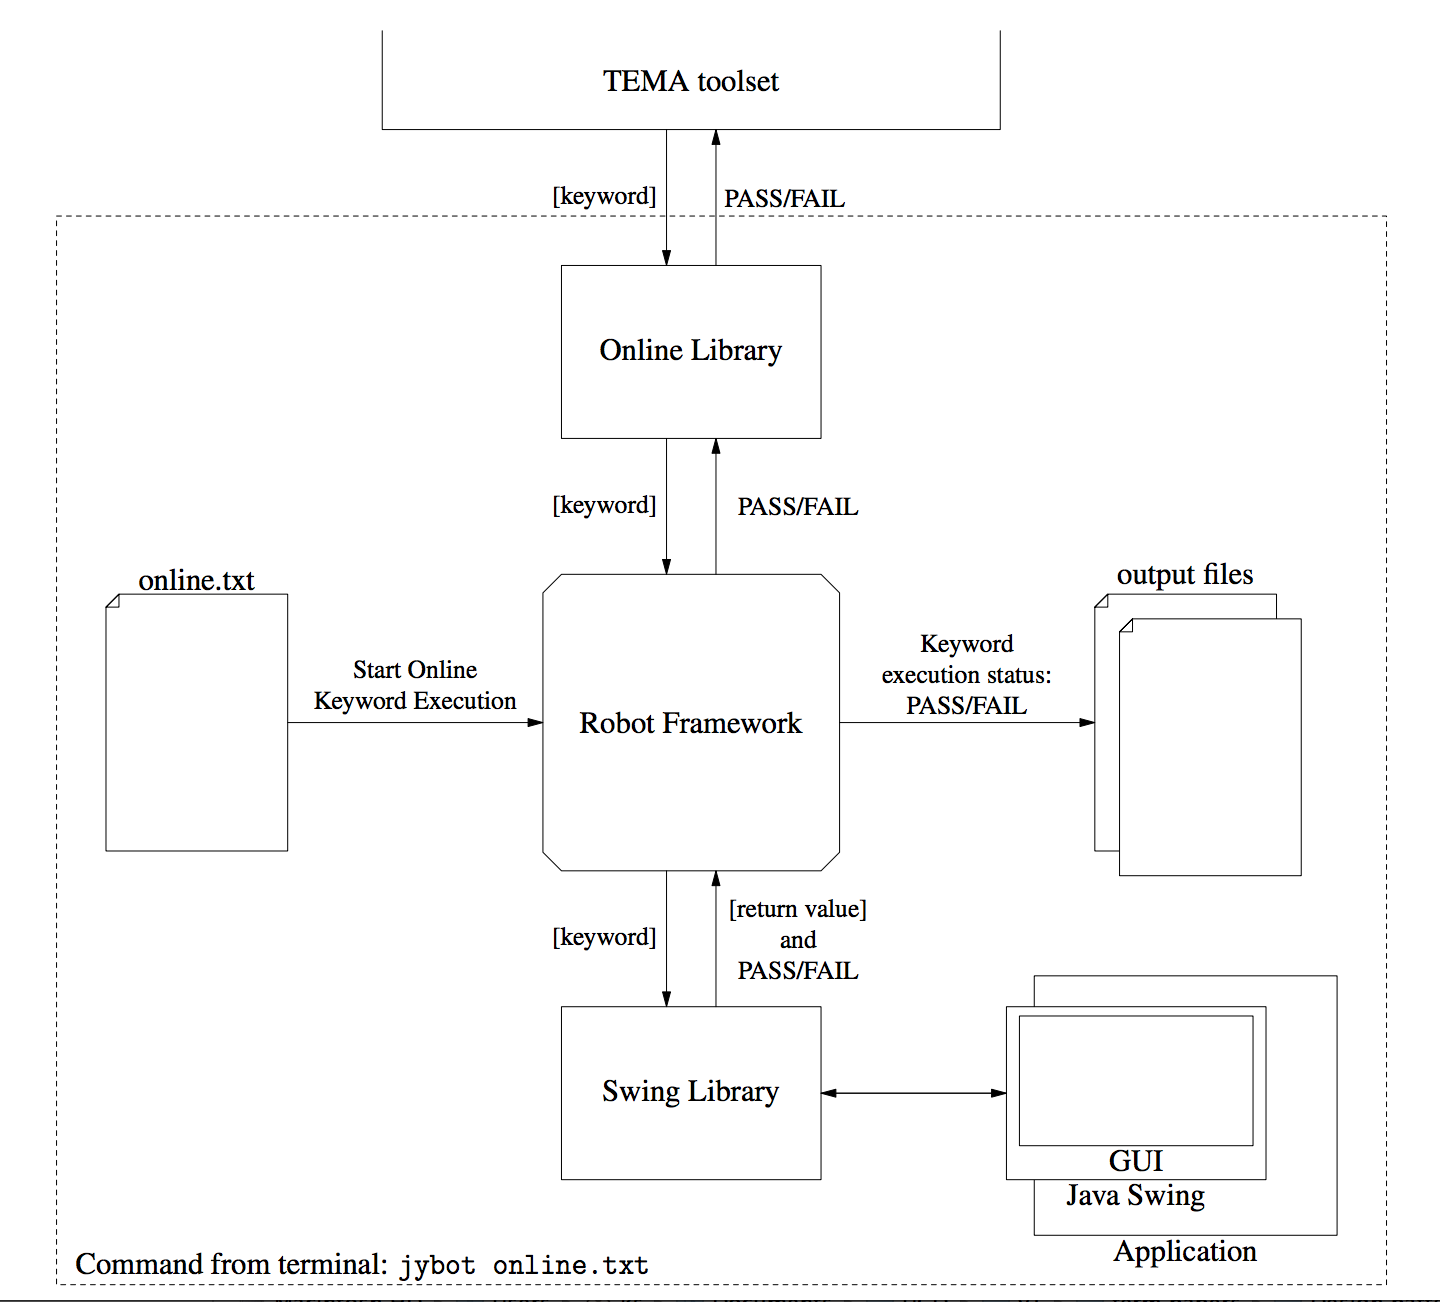
\includegraphics[width=160mm, height=140mm]{robot_tema_int.png}
\caption{TEMA and Robot Framework integration ~\cite{ref:2.1} }
\label{integration}
\end{figure}

\paragraph{Online library}refers to library implemented for integration purposes -- uses the internal structures of Robot framework to parse and execute the received keyword and then passes the keyword execution result to the TEMA toolset. To handle execution result exchange between \emph{Online library} and test engine, authors of the paper implemented \emph{Adapter unit}. For detailed information refer to
~\cite{ref:2.1}.
\paragraph{Keywords} almost all the keywords of the import resource files and the libraries of Robot Framework can be used in testing.

\subsubsection{Make use of the "Repository" pattern to make it easier to create objects}


\subsection{Page Object Pattern}
Page Object pattern is a design pattern used mostly in web application testing. Page Object represents application area that interacts with the test. More specifically, represents a service provided by a particular page. 
Code example for google.com testing:

\begin{verbatim}
class GoogleSearchPage
  def initialize
    @driver = Webdriver.new
    @q = WebElement.new
    @btn = WebElement.new
  end
  def open(url)
    @driver.get url
  end
  def close
    @driver.quit
  end
  def getTitle
    @driver.getTitle
  end
  def searchFor(searchString)
    @q.sendKeys searchString
    @btn.click
  end
  def typeSearchTerm(searchTerm)
    @q.sendKeys searchTerm
  end
  def clickOnSearch
    @btn.click
  end
end
\end{verbatim}


This approach has a number advantages.


\subsection{LoadableComponent}
\subsection{Bot Style Tests}
\subsection{Observer - for AJAX calls}
\subsection{Lazy Initialization}
\subsection{Double Checked Locking}




\begin{thebibliography} {9}
\bibitem{ref:1.1} Eric Evans, {\sl Domain-Driven Design: Tackling Complexity in the Heart of Software}, Addison-Wesley Professional, 2003, ISBN-10: 0-321-12521-5, ISBN-13: 978-0-321-12521-7
\bibitem{ref:2.1} Pajunen, T.; Takala, T.; Katara, M.; {\sl Model-Based Testing with a General Purpose Keyword-Driven Test Automation Framework}, 2011, Fourth International Conference on Software Testing, Verification and Validation Workshops
\bibitem{ref:3.1} Selenium wiki page, \url{https://code.google.com/p/selenium/w/list}
\end{thebibliography}


\end{document}
